\documentclass[abstracton,12pt]{scrartcl}
    
\usepackage[utf8]{inputenc}
% \usepackage[T1]{fontenc}
\usepackage{fancyhdr}
\usepackage{graphicx}
\usepackage{tikz}
\usepackage{listings}
\usepackage{amssymb}
\usepackage{amsfonts}
\usepackage{amsmath}
\usepackage{amsthm}
\usepackage{pdfpages}
\usepackage{forest}
\usepackage{multicol}
\usepackage{varwidth}
\usepackage{verbatim}
%\usepackage{minted}
\usepackage{framed}
\usepackage[ruled,vlined]{algorithm2e}
\usepackage{caption}
\usepackage{subcaption}
\usepackage{cleveref}
\usepackage{soul}
\usepackage{float}
\usepackage{wrapfig}
% \usepackage{geometry}
% \usepackage{titlesec}

% \forestset{qtree/.style={for tree={parent anchor=south, child anchor=north,align=left,inner sep=0pt}}}
\graphicspath{
  {images/},
  {images/1_unprod_nodes/},
  {images/2_unprod_nodes_tau/}
  {images/3_unprod_nodes_L/}
}

% \setlength{\multicolsep}{6.0pt plus 2.0pt minus 1.5pt}% 50% of original values
% \titleformat{\chapter}{}{\thechapter}{}{}
% \titlespacing{\chapter}{-100pt}{-100pt}{-100pt}

% --------- 

\titlehead{Department of Informatics, University of Zürich}
\subject{\vspace*{2cm}BSc Thesis}
\title{An Adaptive Index for Hierarchical Distributed Database Systems}
\author{
    Rafael Kallis\\[-5pt]
    \scriptsize Matrikelnummer: 14-708-887\\[-5pt]
    \scriptsize Email: \texttt{rk@rafaelkallis.com}
}
\date{\vspace*{2cm}February 1, 2018}
\publishers{
    \small supervised by Prof.\ Dr.\ Michael\ Böhlen and Kevin\ Wellenzohn \\[5cm]
    \begin{tikzpicture}[overlay]
    \node at (-3,-3) {
\includegraphics[height=1.5cm]{IFIlogo}};
    \node at (7,-3) {
\includegraphics[height=1.5cm]{dbtgBW}};
    \end{tikzpicture}
}

% \dedication{dedicated to xxx}

% --------- 

\theoremstyle{definition}

\newtheorem{definition}{Definition}
% \newtheorem{figure}{Figure}
\newtheorem{example}{Example}
% \newtheorem{theorem}{Theorem}
% \newtheorem{lemma}{Lemma}

\crefname{algocfline}{algorithm}{algorithms}
\Crefname{algocfline}{Algorithm}{Algorithms}

\crefname{figure}{Fig.}{Figs.}
\Crefname{figure}{Figure}{Figures}

\crefname{example}{Ex.}{Ex.}
\Crefname{example}{Example}{Examples}

% \newenvironment{proof}
%     {\noindent{\bf Proof:\rm}}{\hfill$\Box$\vspace{\medskipamount}}

\newenvironment{centerverbatim}{\par\centering\varwidth{\linewidth}\verbatim}
    {\endverbatim\endvarwidth\par}

% \def\bbbr{{\rm I\!R}}
% \def\bbbm{{\rm I\!M}}
% \def\bbbn{{\rm I\!N}}
% \def\bbbz{{\rm I\!Z}}

\definecolor{shadecolor}{rgb}{0.97,0.97,0.97}
    
\begin{document}

\maketitle
\thispagestyle{empty}
% \chapter*{Acknowledgements}

% \chapter*{Zusammenfassung}
\newpage\null\thispagestyle{empty}\newpage

\tableofcontents
\listoffigures
% \listoftables

\newpage\null\thispagestyle{empty}\newpage

% \begin{abstract}
%   Frequently adding and removing data from hierarchical indexes causes them to
%   repeatedly grow and shrink. A single insertion or deletion can trigger a
%   sequence of structural index modifications (node insertions/deletions) in a
%   hierarchical index. Skewed and update-heavy workloads trigger repeated
%   structural index updates over a small subset of nodes to the index.

%   Informally, a frequently added or removed node is called \textit{volatile}.
%   Volatile nodes deteriorate index update performance due to two reasons.
%   First, frequent structural index modifications are expensive since they
%   cause many disk accesses. Second, frequent structural index modifications
%   also increase the likelihood of conflicting index updates by concurrent
%   transactions. Conflicting index updates further deteriorate update
%   performance since concurrency control protocols need to resolve the
%   conflict.


% \end{abstract}

\section{Introduction}

Frequently adding and removing data from hierarchical indexes causes them to
repeatedly grow and shrink. A single insertion or deletion can trigger a
sequence of structural index modifications (node insertions/deletions) in a
hierarchical index. Skewed and update-heavy workloads trigger repeated
structural index updates over a small subset of nodes to the index.

Informally, a frequently added or removed node is called \textit{volatile}.
Volatile nodes deteriorate index update performance due to two reasons. First,
frequent structural index modifications are expensive since they cause many disk
accesses. Second, frequent structural index modifications also increase the
likelihood of conflicting index updates by concurrent transactions. Conflicting
index updates further deteriorate update performance since concurrency control
protocols need to resolve the conflict.

Wellenzohn et al.~\cite{KW17} propose the Workload-Aware Property Index (WAPI).
The WAPI exploits the workloads' skewness by identifying and not removing
volatile nodes from the index, thus significantly reducing the number of
expensive structural index modifications. Since fewer nodes are
inserted/deleted, the likelihood of conflicting index updates by concurrent
transactions is reduced.

When the workload characteristics change, new index nodes can become volatile
while others cease to be volatile and become \textit{unproductive}. Unproductive
index nodes slow down queries as traversing an unproductive node is useless,
because neither the node itself nor any of its descendants contain an indexed
property and thus cannot yield a query match. Additionally, unproductive nodes
occupy storage space that could otherwise be reclaimed. lf the workload changes
frequently, unproductive nodes quickly accumulate in the index and the query
performance deteriorates over time. Therefore, unproductive nodes must be
cleaned up to keep query performance stable over time and reclaim disk space as
the workload changes.

Wellenzohn et al.~\cite{KW17} propose periodic Garbage Collection (GC), which
traverses the entire index subtree and prunes all unproductive index nodes at
once. Additionally we propose Query-Time Pruning (QTP), an incremental approach
to cleaning up unproductive nodes in the index. The idea is to turn queries into
updates. Since Oak already traverses unproductive nodes as part of query
processing, these nodes could be pruned at the same time. In comparison to GC,
with QTP only one query has to traverse an unproductive node, while subsequent
queries can skip this overhead and thus perform better.

The goal of this BSc thesis is to study, implement, and empirically compare GC
and QTP as proposed by \cite{KW17} in Apache Jackrabbit Oak (Oak).

% The goal of this project is to implement a WAPI, as proposed by \cite{KW17} in
% Apache Jackrabbit Oak (Oak) in order to improve the transactional throughput
% of Oak. In \Cref{sec:wapi} we describe how nodes are inserted, queried and
% deleted from the WAPI. Next, we describe how volatility is computed in
% \Cref{sec:volatility}. Finally, a reference implementation in Java is
% presented in \Cref{sec:implementation}.

\section{Background}

\subsection{Apache Jackrabbit Oak (Oak)}

Oak is a hierarchical distributed database system which makes use of a
hierarchical index. Multiple transactions can work concurrently by making use of
Multiversion Concurrency Control (MVCC)~\cite{GW02}, a commonly used optimistic
concurrency control technique~\cite{TM11}.

\Cref{fig:architecture} depicts Oak's multi-tier architecture. Oak embodies the
\textit{Database Tier}. Multiple Oak instances can operate concurrently.
Whilst Oak is responsible for handling the database logic, it stores the actual
data on MongoDB\footnote{https://www.mongodb.com/what-is-mongodb}, labeled as
\textit{Persistence Tier}. On the other end, applications can make use of Oak as
shown in \Cref{fig:architecture} under \textit{Application Tier}.
One such application is Adobe's enterprise content management system (CMS),
the Adobe Experience
Manager\footnote{http://www.adobe.com/marketing-cloud/experience-manager.html}.

% \begin{wrapfigure}{r}{0.5\textwidth}
\begin{figure}[h]
  \begin{center}
    \begin{tikzpicture}[scale=0.8,thick]
	    \node (mongo) at (0, 0) {
\includegraphics[width = 0.7cm]{MONGO}}; \node
      (oak_a) at (-2, 2) {
\includegraphics[width = 0.7cm]{OAK}}; \node (oak_b)
      at (0, 2) {
\includegraphics[width = 0.7cm]{OAK}}; \node (oak_c) at (2, 2)
      {
\includegraphics[width = 0.7cm]{OAK}}; \node (app_a) at (-2, 4)
      {
\includegraphics[width = 0.7cm]{AEM}}; \node (app_b) at (0, 4)
      {
\includegraphics[width = 0.7cm]{AEM}}; \node (app_c) at (2, 4)
      {
\includegraphics[width = 0.7cm]{AEM}}; \node (mongo_desc) at (5, 0)
      {\footnotesize \textit{Persistence Tier}}; \node (oak_desc) at (5, 2)
      {\footnotesize \textit{Database Tier}}; \node (mongo_desc) at (5, 4)
      {\footnotesize \textit{Application Tier}}; \foreach \from/\to in
      {app_a/oak_a, app_b/oak_b, app_c/oak_c, oak_a/mongo, oak_b/mongo,
        oak_c/mongo} \draw [->] (\from) -- (\to);
    \end{tikzpicture}
  \end{center}
  % \vspace{-0.5cm}
  \caption{Oak's system architecture}
  \label{fig:architecture}
  % \end{wrapfigure}
\end{figure}

\subsection{Application Scenario}
\label{sec:application_scenario}

Content management systems that make use of Oak have specific workloads.
These workloads have distinct properties: they are \textit{skewed},
\textit{update-heavy}, \textit{changing} \cite{KW17} and
\textit{job-queue} like.

Consider a social media feed as a running example. When
browsing the feed, more recent posts are displayed first, therefore creating a
skewed workload. Users submit new posts or interact with existing posts by
writting comments for example, creating an update-heavy workload. As time
passes, new posts are created. Users are more likely to interact with recent
posts than older ones, making the workload change over time.

When a user submits a new post, it is sent to the CMS for processing. A
background thread is periodically checking for pending jobs. A pending job is
signalled using node properties in Oak.
The CMS adds a ``pub'' property with value ``now'' to the respective node  in
order to signal the background thread that the specific node is a pending job that needs
processing. Once the
background thread detects the node and finishes processing, it removes the ``pub'' property and
successfully publishes the post. Informally, we call such a workload
job-queue like.

From now on, we refer to a workload with the properties mentioned above, as
a \textit{CMS workload}.

\subsection{Workload Aware Property Index (WAPI)}
\label{sec:wapi}

Oak mostly executes content-and-structure (CAS) queries~\cite{CM15}.
We denote node $n$'s property $k$ as $n[k]$ and node $n$'s desendants as
$desc(n)$.

\begin{definition}[CAS Query]
  Given content node $m$, property $k$ and value $v$, a CAS query
  $Q(k,v,m)$ returns all descendants of $m$ which have $k$ set to $v$, i.e
  $$ Q(k,v,m) = \{ n | n \in desc(m) \land n[k] = v\} $$
\end{definition}

The WAPI is an hierarchical index and indexes the properties of nodes in order
to answer CAS queries efficiently.
The WAPI is hierarchically organized under node \texttt{/i} (denoted
\textit{Index Subtree Root} in \Cref{fig:hierarchical_db}).
The second index level consists of all properties $k$ we want
to index. The third index level contains any values $v$ of property $k$.
The remaining index levels replicate all nodes from the root node to any
content node with $k$ set to $v$.

\begin{example}[CAS Query]
  Consider \Cref{fig:hierarchical_db}. CAS-Query $Q(\text{pub},\text{now},\texttt{/a})$,
  which queries for every descendant of \texttt{/a} with
  ``pub'' set to ``now'', would evaluate to $Q(\text{pub},\text{now},\texttt{/a}) = \{\texttt{/a/b/d}\}$,
  since \texttt{/a/b/d} is the only descendant of \texttt{/a} with ``pub'' set
  to ``now''.
\end{example}

When processing a CAS Query, Oak traverses the WAPI in order to answer the query
efficiently. Any index node has a \textit{corresponding} content node.
Given index node $n$, we denote $n$'s corresponding content node as $*n$.
If index node $n$'s path is $path(n) = \texttt{/i/k/v/m}$, then $n$'s corresponding content
node $*n$ must have path $path(*n) = \texttt{m} = \texttt{/}\lambda_1\texttt{/}\dots\texttt{/}\lambda_d$.

\begin{figure}
  \centering
  \scriptsize{
    \begin{forest}
      [
      [$\lambda:i$
      [$\lambda:\text{pub}$
      [$\lambda:\text{now}$
      [$\lambda:a$
      [$\lambda:b$
      [$\lambda:d$ \\ $\text{pub}:\text{now}$, align=center, base=bottom, name=i_node] {
        \draw[<-,gray] (.north west)--++(-5em,1em)
        node[anchor=east]{\textit{Matching Node}};
      }
      ]
      [,phantom]
      ]
      ]
      ]
      ] {
        \draw[<-,gray] (.south west)--++(-5em, -1em)
        node[anchor=east]{\textit{Index Subtree Root}};
      }
      [$\lambda:a$
      [$\lambda:b$
      [$\lambda:d$ \\ $\text{pub}:\text{now}$, align=center, base=bottom, name=c_node]
      ]
      [$\lambda:c$
      [$\lambda:e$]
      ]
      ] {
        \draw[<-,gray] (.south east)--++(5em, -1em)
        node[anchor=west]{\textit{Content Subtree Root}};
      }
      ]
      \draw[->,dotted] (i_node) to[out=east, in=south] node[gray,midway,right]{\textit{corresponding content node}} (c_node);
    \end{forest}
  }
  \caption{An instance of an hierarchical database}
  \label{fig:hierarchical_db}
\end{figure}

\begin{definition}[Matching Node]
  Index node $n$, with path \texttt{/i/k/v/m}, is matching
  iff $n$'s corresponding content node $*n$, with path \texttt{m}, has property
  \texttt{k} set to \texttt{v}, i.e
  $$ matching(n) \iff *n[k] = v $$
  \label{def:matching_node}
\end{definition}

\begin{example}[Matching Node]
  Consider \Cref{fig:hierarchical_db}. The subtree rooted at \texttt{/a} is
  the content subtree. The subtree rooted at \texttt{/i} is the index
  substree. Node \texttt{/i/pub/now/a/b/d} is matching, since its corresponding
  content node, \texttt{/a/b/d}, has property ``pub'' set to ``now''.
\end{example}

As mentioned in \Cref{sec:application_scenario}, the CMS workload has certain
properties. From the workload we can infer that the index subtree has a small number of
matching nodes relative to the content subtree. The index is
 used to signal pending jobs to the background thread using
the ``pub'' property. Assuming jobs are processed by
the background thead faster and removed from the index than they are created,
the number of matching nodes should be close to $0$.  

The CMS workload is also skewed and update-heavy, therefore causing repeated structural index
updates over a small subset of nodes to the index.
The WAPI takes into account if an index node is frequently added and removed,
i.e \textit{volatile} (see \Cref{def:volatile_node}), before performing structural
index modifications. If a node is considered volatile, we do not remove it from the index.

Volatility is the measure which is used by the WAPI in order to distinguish
when to remove a node or not from the index.
Wellenzohn et al.~\cite{KW17} propose to look at the recent transactional
workload to check whether a node $n$ is volatile. The workload on Oak instance
$O_i$ is represented by a sequence $H_i = \langle \ldots, G^a, G^b, G^c
\rangle$ of snapshots, called a history. A snapshot represents an immutable
commited tree of the datbase. Let $t_n$ be the current time and
$t(G^b)$ be the point in time snapshot $G^b$ was committed, $N(G^a)$ is the
set of nodes which are members of snapshot $G^a$. We use a superscript $a$
to emphasize that a node $n^a$ belongs to tree $G^a$. $pre(G^b)$ is the
predecessor of snapshot $G^b$ in $H_i$.

Node $n$ is volatile iff $n$'s volatility count is at least $\tau$, called
volatility threshold. The volatility count of $n$ is defined as the number of
times $n$ was added or removed from snapshots in a sliding window of length
$L$ over history $H_i$.

Given two snapshots $G^a$ and $G^b$ we write $n^a$ and $n^b$ to emphasize that
nodes $n^a$ and $n^b$ are two versions of the same node $n$, i.e, they have
the same absolute path from the root node.

\begin{definition}[Volatility Count]
  The volatility count $vol(n)$ of index node $n$ on Oak instance $O_i$, is the number of
  times node $n$ was added or removed from snapshots contained in a sliding
  window of length $L$ over history $H_i$.
  \begin{align*}
    vol(n) = | \{ G^b | G^b \in H_i \land t(G^b) \in [t_{n-L+1}, t_n] \land \exists G^a[ \\
    \qquad G^a = pre(G^b) \land ([n^a \notin N(G^a) \land n^b \in N(G^b)]\lor \\
    \qquad [n^a \in N(G^a) \land n^b \notin N(G^b)] )]\} |
  \end{align*}
  \label{def:vol_count}
\end{definition}

\begin{definition}[Volatile Node]
  Index node $n$ is volatile iff $n$'s volatility count (see
  \Cref{def:vol_count}) is greater or equal than the volatility threshold
  $\tau$, i.e
  $$ volatile(n) \iff vol(n) \geq \tau $$
  \label{def:volatile_node}
\end{definition}

\begin{example}[Volatile Node]
  Consider the snapshots depicted in \Cref{fig:unproductive_nodes}. Assume volatility
  threshold $\tau = 1$, sliding window length $L = 1$ and history $H_h
  = \langle G^0,G^1,G^2,G^3 \rangle$. Oak instance $O_h$ executes transactions
  $T_1, \dots , T_3$. Snapshot $G^0$ was committed at time $t(G^0) =
  t$. Given snapshot $G^0$, transaction $T_1$ adds property ``pub'' = ``now'' to
  \texttt{/a/b/d} and commits snapshot $G^1$ at time $t(G^1) = t + 1$. Next,
  transaction $T_2$ removes property ``pub'' from \texttt{/a/b/d} given snapshot
  $G^1$ and commits snapshot $G^2$ at time $t(G^2) = t + 2$. The index nodes are
  not pruned during $T_2$ since they are volatile.
  \label{ex:volatile_node}
\end{example}

\begin{figure}[h]
  \centering

  \begin{large}
    $$ G^0 \xrightarrow{\quad T_1 \quad} G^1 \xrightarrow{\quad T_2 \quad} G^2
    \xrightarrow{\quad T_3 \quad} G^3  $$
  \end{large}

  \begin{subfigure}{0.24\textwidth}
    \centering \tiny{
      \begin{framed}
        \begin{forest}
        [
        [$\lambda$:$i$
        [,phantom]
        ]
        [,phantom]
        [,phantom]
        [$\lambda$:$a$
        [$\lambda$:$b$
        [$\lambda$:$d$]
        ] 
        [,phantom]
        [$\lambda$:$c$
        [$\lambda$:$e$]
        ]
        ]
        ]
      \end{forest}

      \vspace{22mm}
    \end{framed}
  } \footnotesize{ Snapshot $G^0$
 
    $t(G^0) = t$ }
\end{subfigure}
\begin{subfigure}{0.24\textwidth}
  \centering \tiny{
    \begin{framed}
      \begin{forest}
        [
        [$\lambda$:$i$
        [$\lambda$:pub
        [$\lambda$:now
        [$\lambda$:$a$
        [$\lambda$:$b$
        [$\lambda$:$d$ \\ pub:now, align=center, base=bottom]
        ]
        [,phantom]
        ]
        ]
        ]
        ]
        [$\lambda$:$a$
        [$\lambda$:$b$
        [$\lambda$:$d$ \\ pub:now, align=center, base=bottom]
        ]
        [$\lambda$:$c$
        [$\lambda$:$e$]
        ]
        ]
        ]
      \end{forest}
    \end{framed}
  } \footnotesize{ Snapshot $G^1$
 
    $t(G^1) = t+1$ }
\end{subfigure}
\begin{subfigure}{0.24\textwidth}
  \centering \tiny{
    \begin{framed}
      \begin{forest}
        [
        [$\lambda$:$i$
        [$\lambda$:pub
        [$\lambda$:now
        [$\lambda$:$a$
        [$\lambda$:$b$
        [$\lambda$:$d$]
        ]
        [,phantom]
        [,phantom]
        ]
        ]
        ]
        ]
        [$\lambda$:$a$
        [$\lambda$:$b$
        [$\lambda$:$d$]
        ]
        [,phantom]
        [$\lambda$:$c$
        [$\lambda$:$e$]
        ]
        ]
        ]
      \end{forest}

      \vspace{3mm}
    \end{framed}
  } \footnotesize{ Snapshot $G^2$
 
    $t(G^2) = t+2$ }
\end{subfigure}
\begin{subfigure}{0.24\textwidth}
  \centering \tiny{
    \begin{framed}
      \begin{forest}
        [
        [$\lambda$:$i$
        [$\lambda$:pub
        [$\lambda$:now
        [$\lambda$:$a$
        [$\lambda$:$b$
        [$\lambda$:$d$]
        ]
        [$\lambda$:$c$
        [$\lambda$:$e$ \\ pub:now, align=center, base=bottom]
        ]
        ]
        ]
        ]
        ]
        [,phantom]
        [$\lambda$:$a$
        [$\lambda$:$b$
        [$\lambda$:$d$]
        ]
        [$\lambda$:$c$
        [$\lambda$:$e$ \\ pub:now, align=center, base=bottom]
        ]
        ]
        ]
      \end{forest}
    \end{framed}
  } \footnotesize{ Snapshot $G^3$
 
    $t(G^3) = t+3$ }
\end{subfigure}

\vspace{3mm}
\caption*{
  Given $\tau = 1$, $L = 1$, nodes \texttt{/i/pub/now/a/b/d} and \texttt{/i/pub/now/a/b}
  are unproductive in snapshot $G^3$. They are not volatile and don't match either.
}
\caption{Volatile nodes becoming unproductive}
\label{fig:unproductive_nodes}
\end{figure}

\section{Unproductive Nodes}

When time passes and the database workload changes, volatile nodes cease to be
volatile and they become unproductive. Unproductive index nodes slow down
queries as traversing an unproductive node is useless, because neither the node
itself nor any of its descendants contain an indexed property and thus cannot
yield a query match. Additionally, unproductive nodes occupy storage space that
could otherwise be reclaimed. If the workload changes frequently, unproductive
nodes quickly accumulate in the index and the query performance deteriorates
over time \cite{KW17}.

\begin{definition}[Unproductive Node]
  Index node $n$ is unproductive iff $n$, and any descendant of
  $n$, is neither matching (see \Cref{def:matching_node}) nor volatile (see
  \Cref{def:volatile_node}), i.e
  $$ unproductive(n) \iff \nexists m (m \in (\{n\} \cup desc(n)) \land
  (matching(m) \lor volatile(m)))$$
\end{definition}

\begin{example}
  In our running example (cf. \Cref{fig:unproductive_nodes}), transaction $T_3$ adds
  property ``pub'' = ``now'' to \texttt{/a/c/e} given $G^2$ and commits $G^3$ at time
  $t(G^3) = t+3$. \texttt{/i/pub/now/a/b/d} and \texttt{/i/pub/now/a/b} are
  the only unproductive index nodes. \texttt{/i/pub/now/a/c/e} and
  \texttt{/i/pub/now/a/c} are the only volatile nodes in $G^3$.
\end{example}

\subsection{Impact on Query Execution Runtime}

In this section we study and quantify the impact of unproductive nodes on
query runtime. Informally, we call \textit{Query Runtime} the time
needed for a query to finish processing. We hypothesize that unproductive nodes
significantly slow down queries under a CMS workload. During query
execution, traversing an unproductive node is
useless, because neither the node itself nor any of its descendants are matching
and therefore cannot contribute a query match.
An index under a CMS workload (see \Cref{sec:application_scenario}) is dominated
by unproductive nodes.

We formalize the statements above into the following hypotheses:

\begin{shaded}
  \begin{itemize}
  \item[$H_1$:] WAPI's average query runtime increases over time under a CMS workload.
  \item[$H_2$:] Unproductive nodes significantly affect WAPI's query runtime
    under a CMS workload. 
  \end{itemize}
\end{shaded}

In order to find supporting evidence for the hypotheses above, we conduct a series of
experiments on Oak. The experimental evaluation and
datasets will be described in a later section (\textbf{forward reference}). We
record the query runtime throughout the experiment and present the data below.

\begin{figure}
  \centering
  \begin{subfigure}{0.49\linewidth}
    \centering
    Synthetic
  \end{subfigure}
  \begin{subfigure}{0.49\linewidth}
    \centering
    Real World
  \end{subfigure}
  \begin{subfigure}{0.49\linewidth}
    \centering
    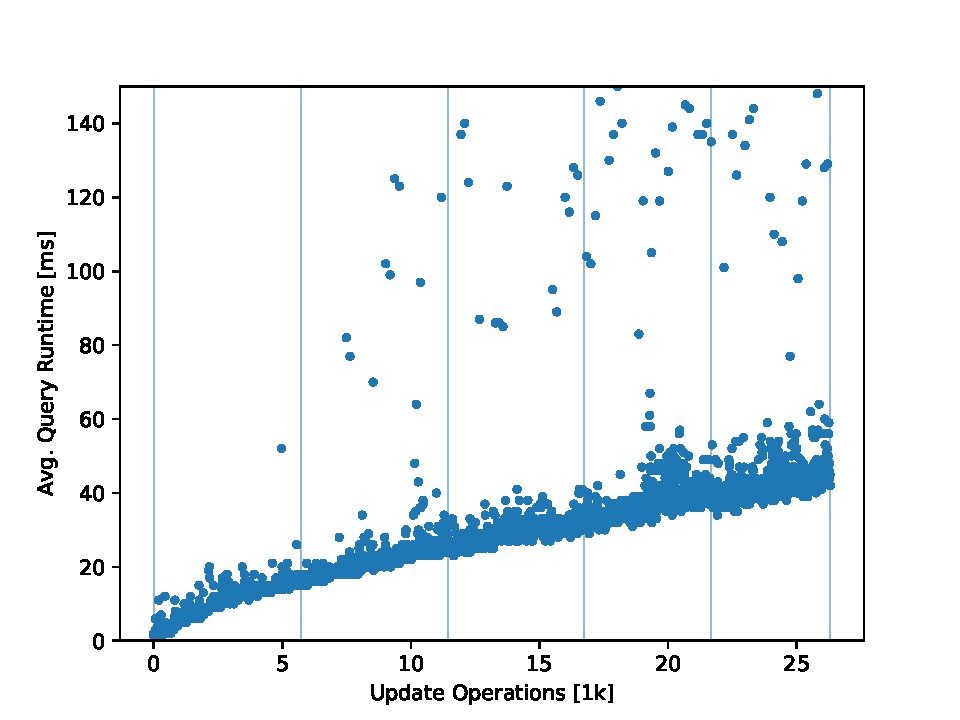
\includegraphics[width=8cm]{query_runtime_synthetic}
    \caption{}
    \label{fig:query_runtime_synthetic}
  \end{subfigure}
  \begin{subfigure}{0.49\linewidth}
    \centering
    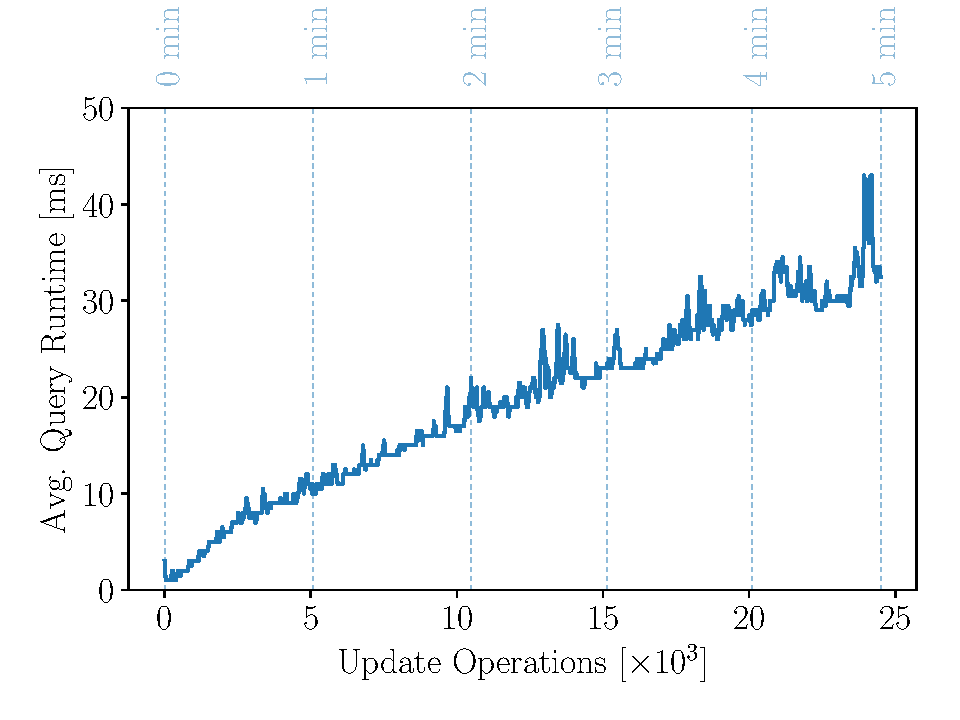
\includegraphics[width=8cm]{query_runtime_real}
    \caption{}
    \label{fig:query_runtime_real}
  \end{subfigure}
  \caption{Query Runtime over time}
  \label{fig:query_runtime}
\end{figure}

\Cref{fig:query_runtime_synthetic,fig:query_runtime_real} show 
query runtime over time from the synthetic and real world dataset respectively. 
Each point corresponds to the moving median over 10 time points.
We observe an increase of the runtime from $2 ms$ to $50 ms$
after running the simulation for $5$ minutes ($2.6 \cdot 10^4$ update operations)
on the synthetic dataset and an increase from $2 ms$ to $35 ms$ ($2.5 \cdot
10^4$ update operations) on the real world dataset.
We also see the slope decrease over time. The identical phenomenon is observed
in \Cref{fig:trav_nodes_synthetic,fig:trav_nodes_real} respectively because
query runtime depends on the number of nodes traversed during query execution,
i.e the increase in query runtime is explained by the increase in total
traversed nodes per query. 

\begin{figure}
  \centering
  \begin{subfigure}{0.49\linewidth}
    \centering
    Synthetic
  \end{subfigure}
  \begin{subfigure}{0.49\linewidth}
    \centering
    Real World
  \end{subfigure}
  \begin{subfigure}{0.49\linewidth}
    \centering
    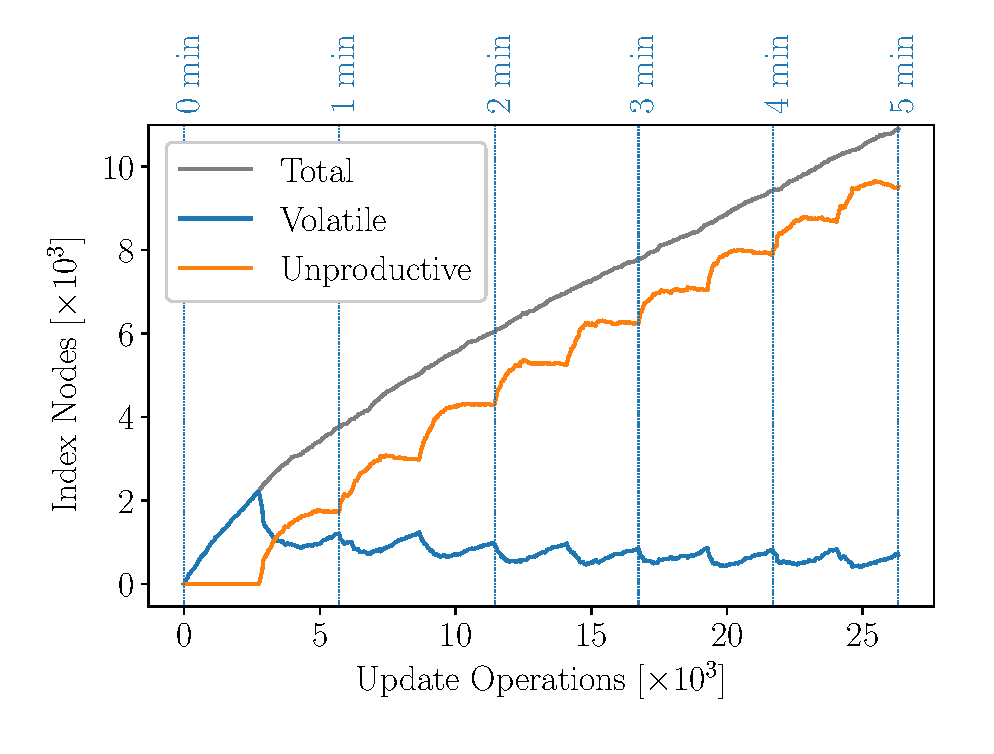
\includegraphics[width=8cm]{trav_nodes_synthetic}
    \caption{}
    \label{fig:trav_nodes_synthetic}
  \end{subfigure}
  \begin{subfigure}{0.49\linewidth}
    \centering
    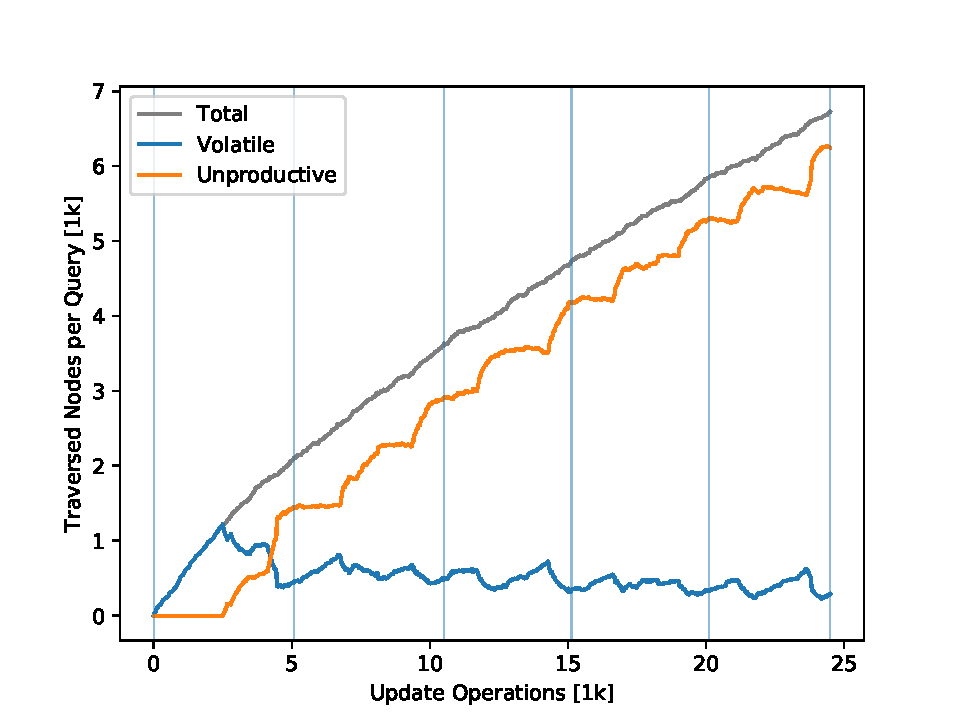
\includegraphics[width=8cm]{trav_nodes_real}
    \caption{}
    \label{fig:trav_nodes_real}
  \end{subfigure}
  \caption{Index Structure during Query Execution}
  \label{fig:trav_nodes}
\end{figure}

Next, we present data regarding the type of index nodes traversed during query
execution.
\Cref{fig:trav_nodes_synthetic,fig:trav_nodes_real} depict
the number of traversed volatile and unproductive index nodes during query
execution for each dataset.

The total number of traversed nodes is increasing over time but the rate of
growth is decreasing. As time passes, more and more content nodes are randomly
selected by the CMS workload and become volatile and, most likely, become
unproductive and are not pruned from the index anymore.
Therefore, the probability of picking a non-indexed content node
decreases over time. Since it becomes less and less likely for a non-indexed content node
to be randomly picked by the CMS workload, the rate of growth of total traversed
index nodes decreases over time.

The sliding window of length $L$ is set to $30$ seconds, therefore we encounter no
unproductive nodes during the first $30$ seconds of the simulation. Once we
reach the $30$ second mark, our queries encounter unproductive nodes.
From that point, we observe a steep increase in traversed unproductive nodes.
After $3$ minutes, we observe the traversed nodes being dominated by
unproductive nodes. The rate of growth of traversed unproductive nodes seems to
decrease over time, which can be explained by the same rationale that cause the
decrease of the rate of growth of total index nodes.

Additionally, we observe a
cycloid shaped curve. In \Cref{fig:trav_nodes_synthetic}, each cusp ($30, 60,
\dots, 300 s$) represents a point in which the workload changes during the
experiment. When the workload changes, we initially see a steep increase in
unproductive nodes. During that phase, more nodes cease to be volatile than
become volatile. Nodes need to reach the threshold in order to become volatile
and relatively few do, since the skew in he workload only picks a subset of
nodes frequently. Before a new workload kicks in, we observe the opposite
phenomenon. More nodes become volatile than cease to be volatile, because many nodes are
on the verge of becoming volatile and therefore need to be picked fewer times to
become volatile in comparison to the time shortly after the workload kicked in. 

The cycloid pattern observed in \Cref{fig:trav_nodes_synthetic} is less obvious
in \Cref{fig:trav_nodes_real}. Our synthetic dataset resembles a complete binary
tree and therefore has no skew. In comparison, the real world dataset is highly
skewed. The skewness warps the shape of the curve inside single workloads,
but does not significantly affect the monotonicity \textbf{(?)} of our function.
We also suggest that the real world dataset's skewness accounts for the lower
rate of growth of index nodes in comparison to the synthetic dataset's rate of
growth of index nodes.

Furthermore, we see the number of volatile nodes descend after the $30$
second mark. We suggest that it becomes less likely for nodes to become volatile,
as time passes. When a workload randomly picks a node whose index node is
unproductive, the index
node becomes matching but was not added, thus the volatility count of the node
does increment. In comparison, if the index node would not exist, the created
index node's volatility count would have been incremented. We infer that it is less
likely for an unproductive node to become volatile than a non-indexed one.
Wellenzohn et al. and our experimental evaluation suggest that the number of
unproductive nodes increases over time. Therefore it becomes less likely for any
node to become volatile over time. This explains the decreasing number of volatile nodes.

\begin{figure}
 \centering
  \begin{subfigure}{0.49\linewidth}
    \centering
    Synthetic
  \end{subfigure}
  \begin{subfigure}{0.49\linewidth}
    \centering
    Real World
  \end{subfigure}
  \begin{subfigure}{0.49\linewidth}
    \centering
    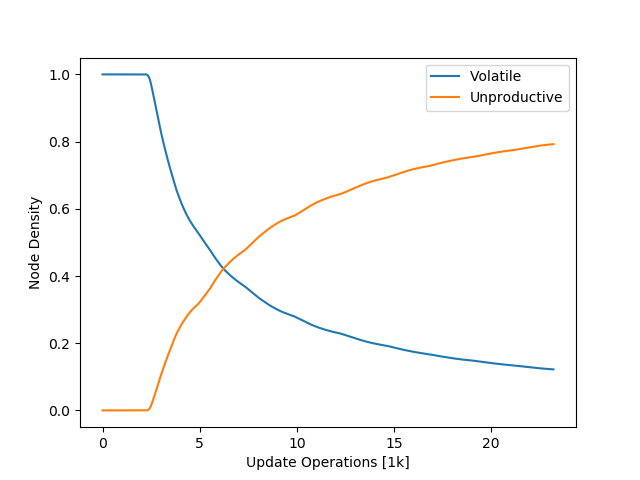
\includegraphics[width=8cm]{trav_node_ratio_synthetic}
    \caption{}
    \label{fig:trav_node_ratio_synthetic}
  \end{subfigure}
  \begin{subfigure}{0.49\linewidth}
    \centering
    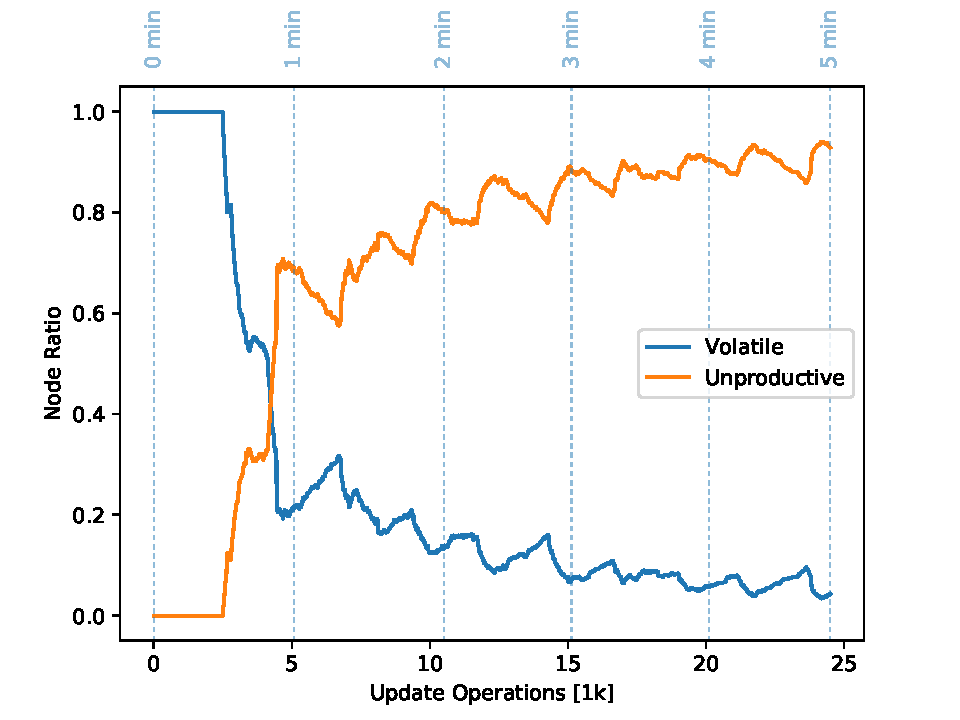
\includegraphics[width=8cm]{trav_node_ratio_real}
    \caption{}
    \label{fig:trav_node_ratio_real}
  \end{subfigure}
  \caption{Node Ratio during Query Execution}
  \label{fig:trav_node_ratio}
\end{figure}

\Crefrange{fig:trav_node_ratio_synthetic}{fig:trav_node_ratio_real}
show the ratio of volatile and unproductive nodes over time and update
operations from our datasets. These figures quantify how strongly unproductive
nodes dominate the traversed nodes. The data shows that unproductive nodes
account for over $80\%$ of the traversed nodes whilst less than $20\%$ are
volatile on the synthetic dataset, $90\%$ and $10\%$ on the real world dataset
respectively.

Concluding, the data strongly supports our hypotheses. We see the query runtime
increase as the number of index nodes increases. We also see unproductive nodes
being mostly accountable for the increase in index nodes. 
In the following sections we will study the effect of \textit{Volatility
  Threshold $\tau$} and \textit{Sliding Window Length $L$} on query runtime and
unproductive nodes.

\subsection{Volatility Threshold $\tau$}

Volatility threshold $\tau$ determines after how many insertions/deletions of an index node
it becomes volatile (see \Cref{def:volatile_node}). In this section, we study the impact of
volatility threshold $\tau$ on unproductive nodes and query runtime.

We hypothesize that an increase in $\tau$ yields a decrease to the number of
traversed unproductive nodes during query execution under a CMS workload. If
$\tau$ increases, it is
less likely for a node to become volatile. Having less volatile nodes should
cause a decrease to the number of unproductive nodes.

An increase in $\tau$ yields a decrease to WAPI's query runtime under a CMS
workload. Having less unproductive nodes in the index decrease the number of nodes traversed
during query execution and therefore decrease query runtime.

\begin{shaded}
  \begin{itemize}
  \item[$H_3$:] An increase in $\tau$ yields a decrease to WAPI's query runtime
    under a CMS workload. 
  \item[$H_4$:] An increase in $\tau$ yields a decrease to the number of
    traversed unproductive nodes during WAPI's query execution under a CMS workload.
  \end{itemize}
\end{shaded}

We conduct the same experiment under a varying volatility threshold. 
\Cref{fig:query_runtime_taus_synthetic,fig:query_runtime_taus_real} show
thresholds $\tau \in \{1,5,10\}$ affecting query runtime
over update operations. We observe that a lower threshold $\tau$ results in a
faster rate of growth of query runtime.
\Cref{fig:tau_query_runtime_synthetic,fig:tau_query_runtime_real} compare query
runtime over a range of thresholds. The values picked correspond to
the query runtime after $10^4$ update operations.
We observe a decrease in query runtime while increasing threshold $\tau$.
Having a lower volatility threshold should increase the likelihood of a node
becoming volatile. The amount of volatile nodes also affect the number of
unproductive nodes, since volatile nodes eventually stop being frequently
updated and become unproductive. The increase in unproductive nodes in the index
directly affects query runtime because Oak has to traverse these nodes during
query execution.

\begin{figure}
  \centering
  \begin{subfigure}{0.49\linewidth}
    \centering
    Synthetic
  \end{subfigure}
  \begin{subfigure}{0.49\linewidth}
    \centering
    Real World
  \end{subfigure}
  \begin{subfigure}{0.49\linewidth}
    \centering
    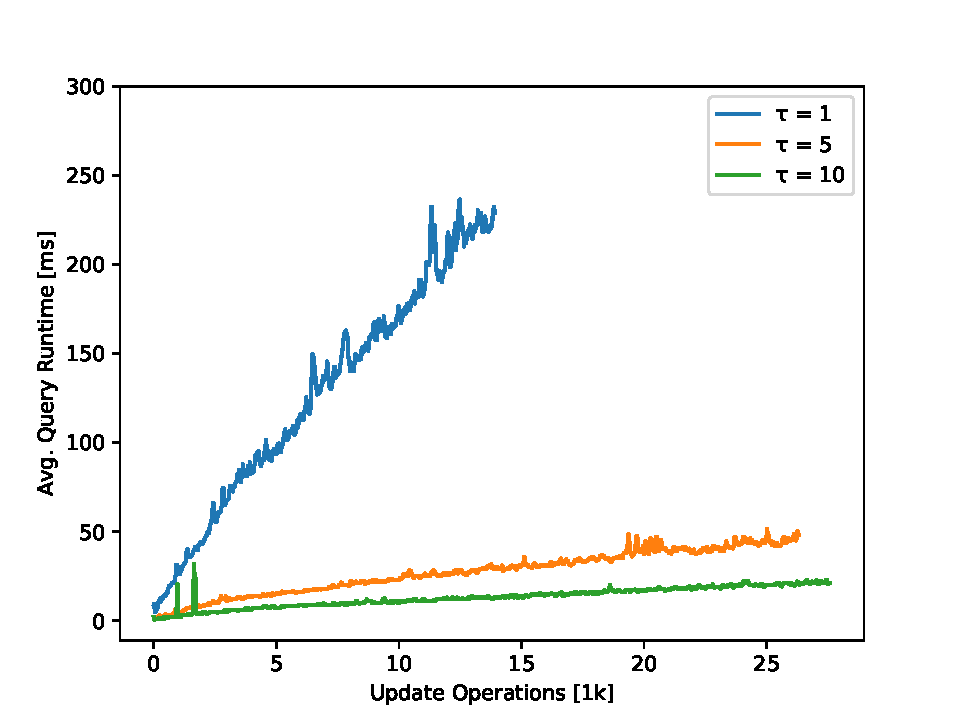
\includegraphics[width=8cm]{query_runtime_taus_synthetic}
    \caption{}
    \label{fig:query_runtime_taus_synthetic}
  \end{subfigure}
  \begin{subfigure}{0.49\linewidth}
    \centering
    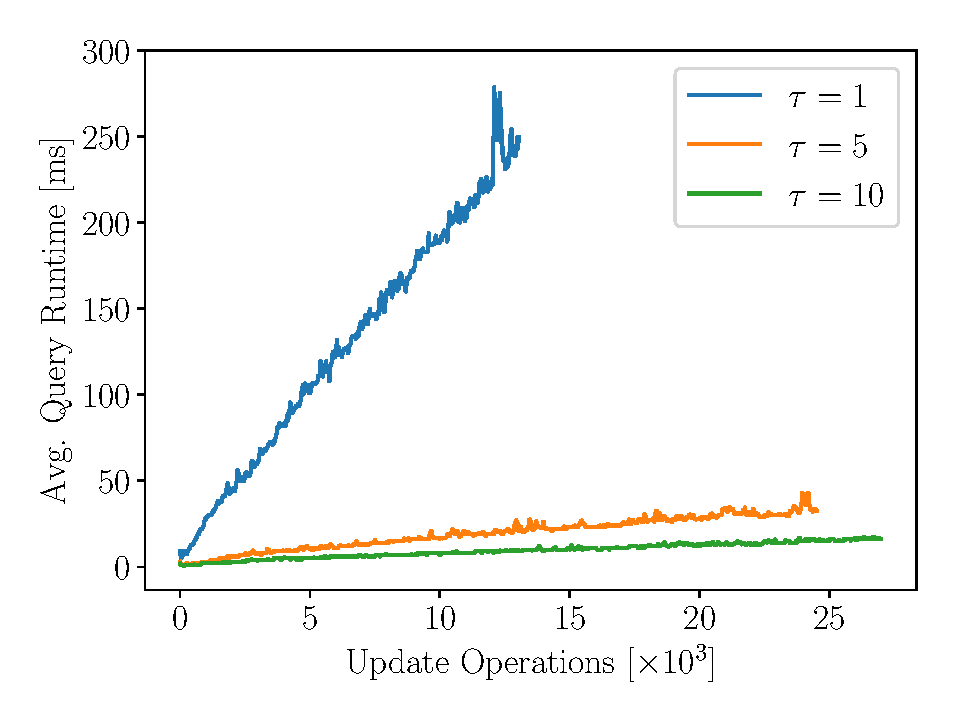
\includegraphics[width=8cm]{query_runtime_taus_real}
    \caption{}
    \label{fig:query_runtime_taus_real}
  \end{subfigure}
  \begin{subfigure}{0.49\linewidth}
    \centering
    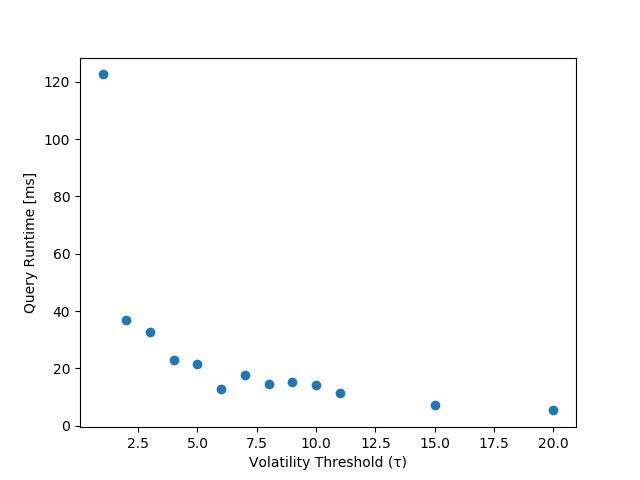
\includegraphics[width=8cm]{tau_query_runtime_synthetic}
    \caption{}
    \label{fig:tau_query_runtime_synthetic}
  \end{subfigure}
  \begin{subfigure}{0.49\linewidth}
    \centering
    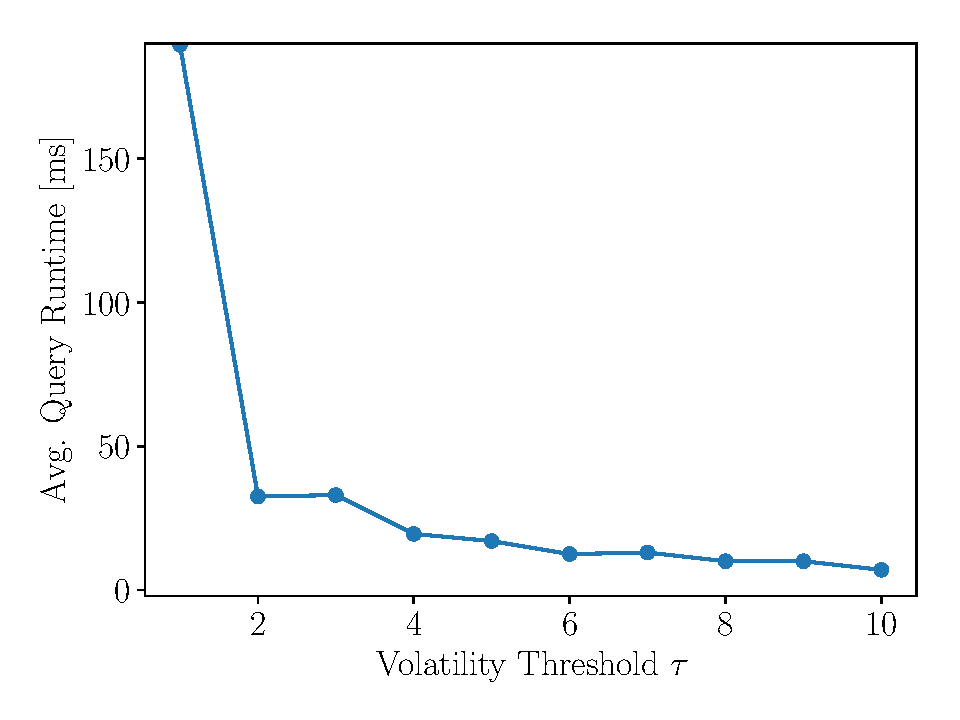
\includegraphics[width=8cm]{tau_query_runtime_real}
    \caption{}
    \label{fig:tau_query_runtime_real}
  \end{subfigure}
\caption{Impact of Volatility Threshold $\tau$ on Query Runtime}
\end{figure}

\Cref{fig:trav_unprod_nodes_taus_synthetic,fig:trav_unprod_nodes_taus_real}
depict thresholds $\tau \in \{1,5,10\}$ affecting the number of unproductive
nodes traversed during query execution over update operations. We observe lower
thresholds $\tau$ yielding in a steeper slope.
\Cref{fig:tau_trav_unprod_nodes_synthetic,fig:tau_trav_unprod_nodes_real} compare the
number of traversed unproductive nodes during query execution over a range of
thresholds. We observe a decrease in unproductive nodes while increasing
threshold $\tau$. As suggested earlier, a lower volatility threshold
increases the amount of volatile nodes in the index. Volatile nodes eventually
cease to be volatile and become unproductive.

\begin{figure}
  \centering
  \begin{subfigure}{0.49\linewidth}
    \centering
    Synthetic
  \end{subfigure}
  \begin{subfigure}{0.49\linewidth}
    \centering
    Real World
  \end{subfigure}
  \begin{subfigure}{0.49\linewidth}
    \centering
    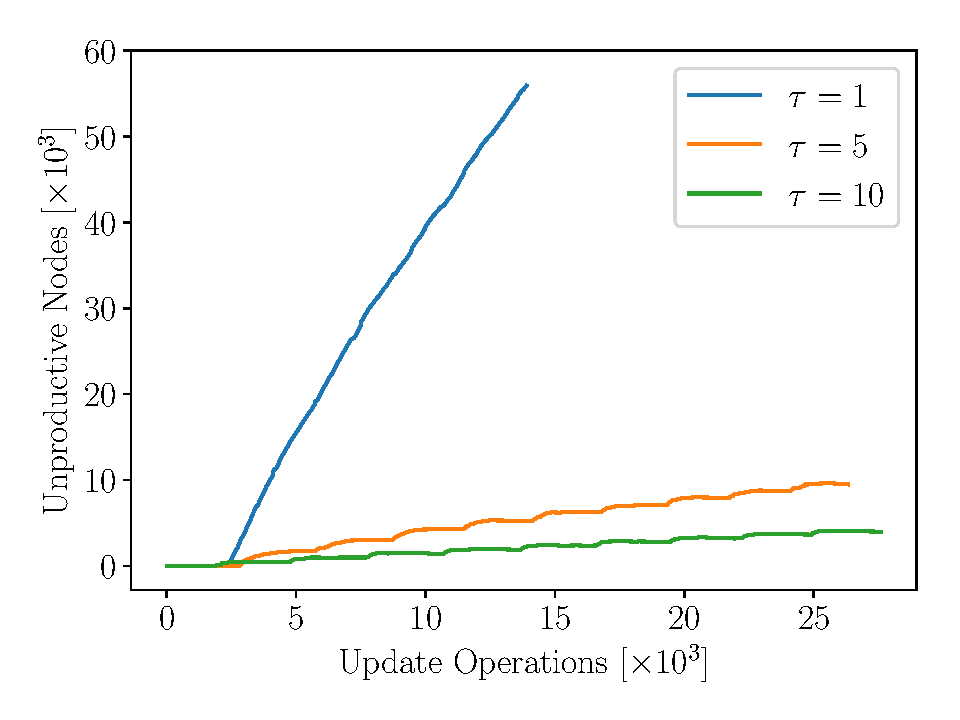
\includegraphics[width=8cm]{trav_unprod_nodes_taus_synthetic}
    \caption{}
    \label{fig:trav_unprod_nodes_taus_synthetic}
  \end{subfigure}
  \begin{subfigure}{0.49\linewidth}
    \centering
    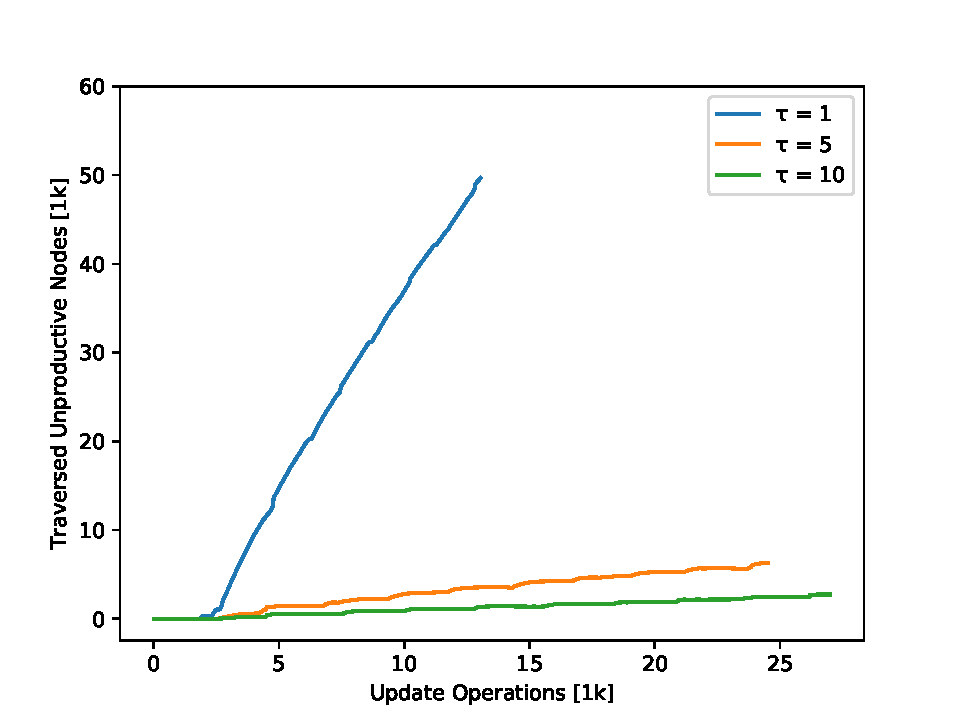
\includegraphics[width=8cm]{trav_unprod_nodes_taus_real}
    \caption{}
    \label{fig:trav_unprod_nodes_taus_real}
  \end{subfigure}
  \begin{subfigure}{0.49\linewidth}
    \centering
    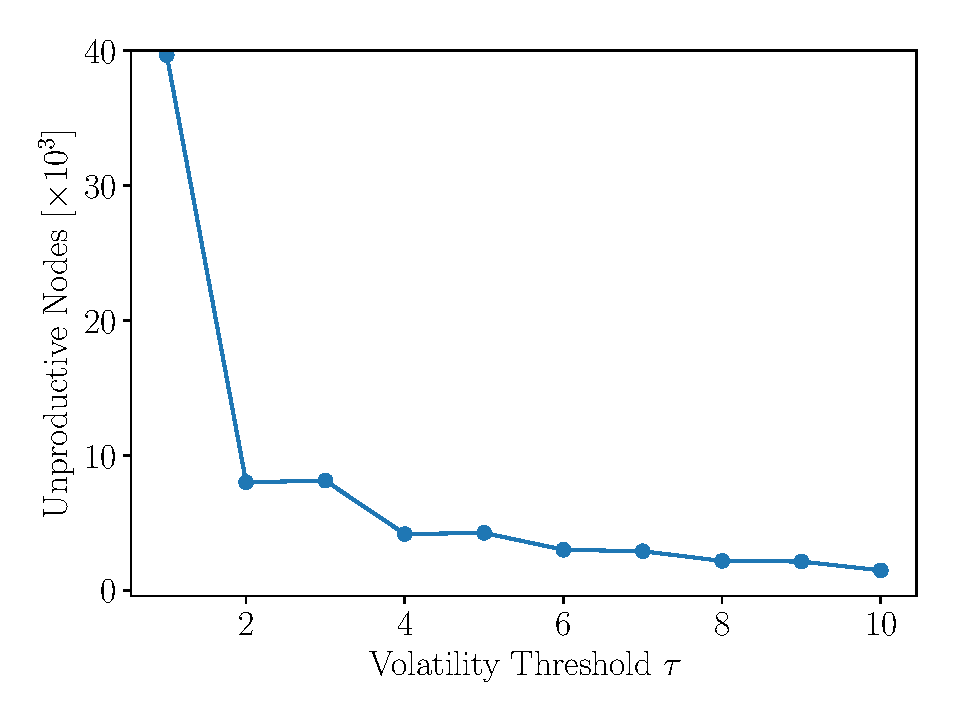
\includegraphics[width=8cm]{tau_unprod_nodes_synthetic}
    \caption{}
    \label{fig:tau_trav_unprod_nodes_synthetic}
  \end{subfigure}
  \begin{subfigure}{0.49\linewidth}
    \centering
    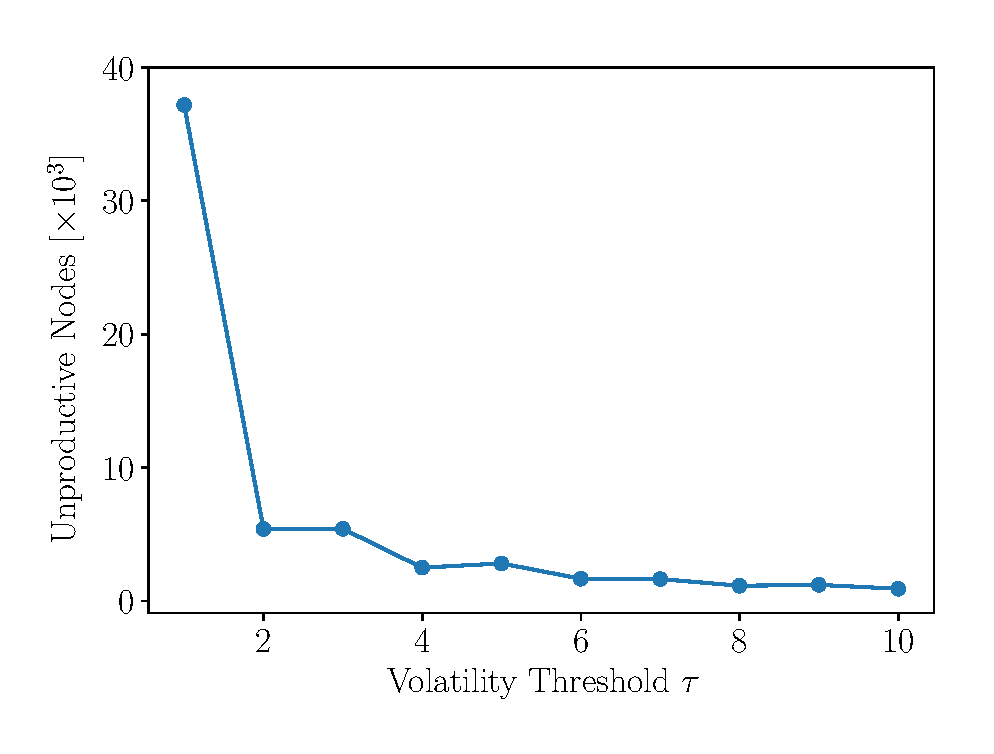
\includegraphics[width=8cm]{tau_unprod_nodes_real}
    \caption{}
    \label{fig:tau_trav_unprod_nodes_real}
  \end{subfigure}
  \caption{Impact of Volatility Threshold $\tau$ on Unproductive Nodes}
\end{figure}

Summarizing, all observations verify hypotheses $H_3$ and $H_4$.
Increasing volatility threshold $\tau$ decreases the number of unproductive
nodes traversed which decreases query runtime. Increasing the volatility
threshold causes less nodes become volatile. Since we create less volatile
nodes, we also reduce the number of unproductive nodes. Less unproductive
nodes yield lower WAPI query runtimes. Another factor affecting the rate of
growth of unproductive nodes is sliding window of length $L$. The following
section addresses the effects of the sliding window.

\subsection{Sliding Window of Length $L$}

Sliding window of length $L$ determines the length of the recent workload that WAPI
considers to compute an index node's volatility count. Greater values of $L$
allow WAPI to consider more updates and therefore increase the chances of a node
becoming volatile. In this section, we study
the effect of the sliding window on unproductive nodes and query runtime.

We hypothesize that an increase in $L$ yields an increase to the number of
traversed unproductive nodes during query execution. If $L$ increases, it is
more likely for a node to become volatile, since more updates are considered
towards the volatility count.
Having more volatile nodes should imply an increase in unproductive nodes.

We also suggest that an increase in $L$ yields an increase to the query runtime.
More unproductive nodes should increase the number of unproductive nodes traversed
during query execution and therefore increase query runtime.

\begin{shaded}
  \begin{itemize}
  \item[$H_5$:] An increase in $L$ yields an increase to WAPI's query runtime
    under a CMS workload. 
  \item[$H_6$:] An increase in $L$ should increase the number of unproductive
    nodes WAPI traverses during query execution under a CMS workload.
  \end{itemize}
\end{shaded}

We conduct our experiment with a varying sliding window length and present our
observations below.

\Cref{fig:query_runtime_Ls_synthetic,fig:query_runtime_Ls_real} show WAPI's average
query runtime over update operations with sliding window of length $L \in \{10, 20,
30\}$ seconds.
\Cref{fig:L_query_runtime_synthetic,fig:L_query_runtime_real} depict query
runtime with respect to the sliding window length. 
We see queries being executed by a WAPI with a greater sliding
window length to have greater runtimes on average. By increasing the sliding
window, we increase the likelihood of a node becoming volatile. More volatile
nodes result in an increase in unproductive nodes. Since the WAPI has to traverse
more unproductive nodes during query execution, the query runtime increases.

\begin{figure}
  \centering
  \begin{subfigure}{0.49\linewidth}
    \centering
    Synthetic
  \end{subfigure}
  \begin{subfigure}{0.49\linewidth}
    \centering
    Real World
  \end{subfigure}
  \begin{subfigure}{0.49\linewidth}
    \centering
    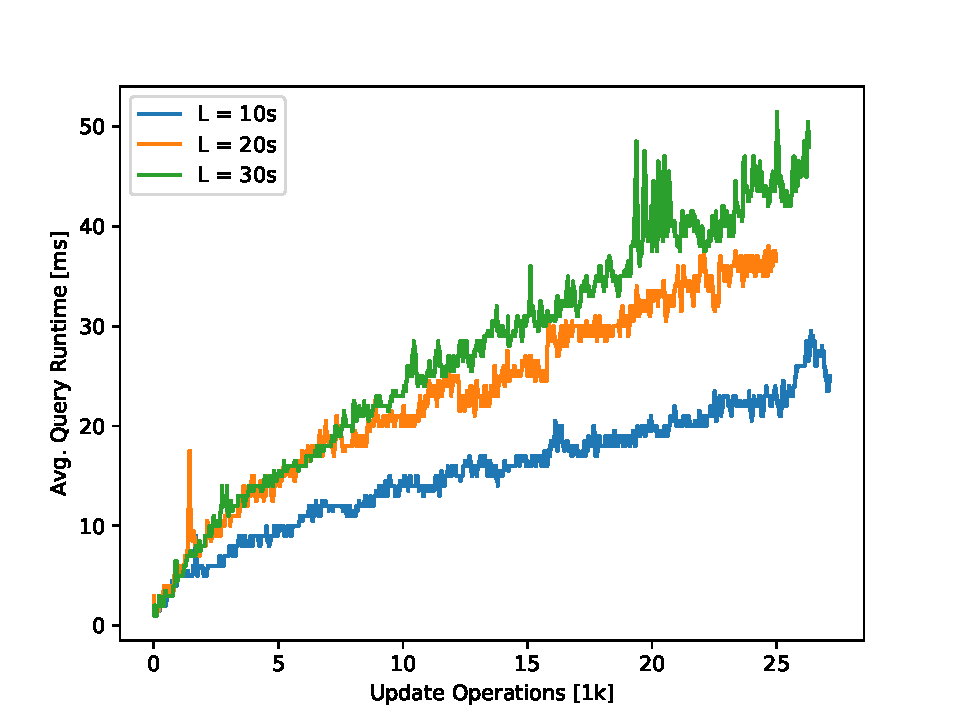
\includegraphics[width=8cm]{query_runtime_Ls_synthetic}
    \caption{}
    \label{fig:query_runtime_Ls_synthetic}
  \end{subfigure}
  \begin{subfigure}{0.49\linewidth}
    \centering
    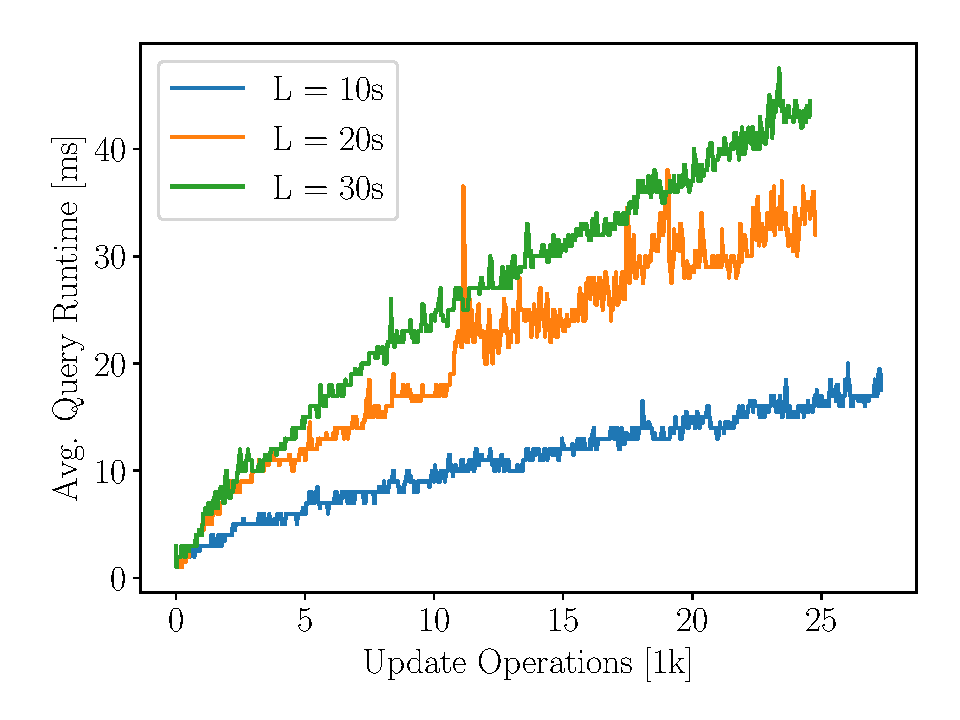
\includegraphics[width=8cm]{query_runtime_Ls_real}
    \caption{}
    \label{fig:query_runtime_Ls_real}
  \end{subfigure}
  \begin{subfigure}{0.49\linewidth}
    \centering
    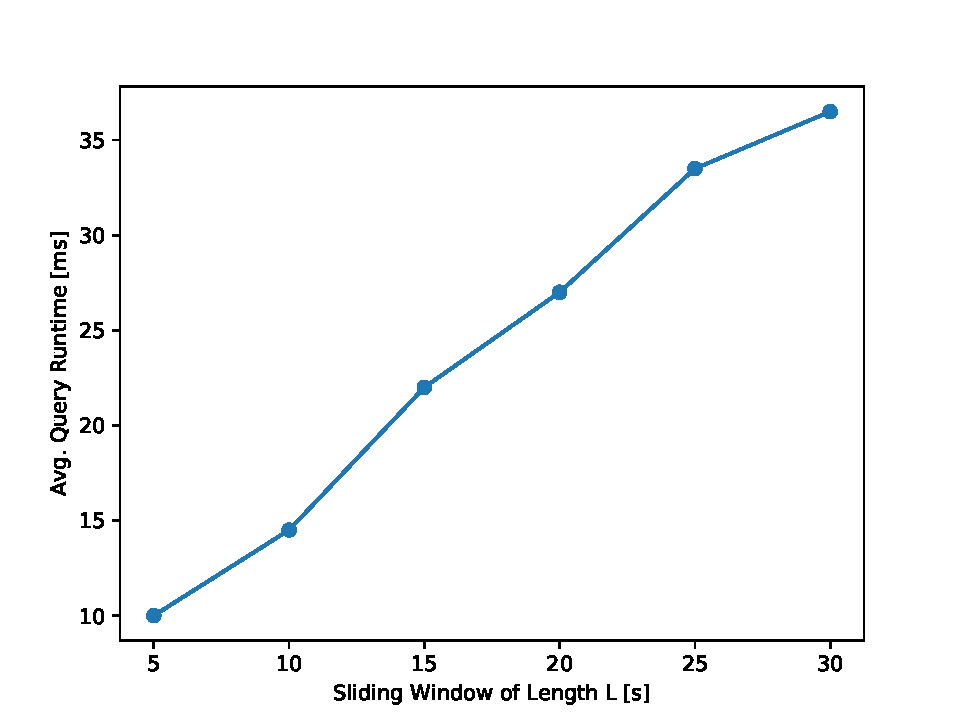
\includegraphics[width=8cm]{L_query_runtime_synthetic}
    \caption{}
    \label{fig:L_query_runtime_synthetic}
  \end{subfigure}
  \begin{subfigure}{0.49\linewidth}
    \centering
    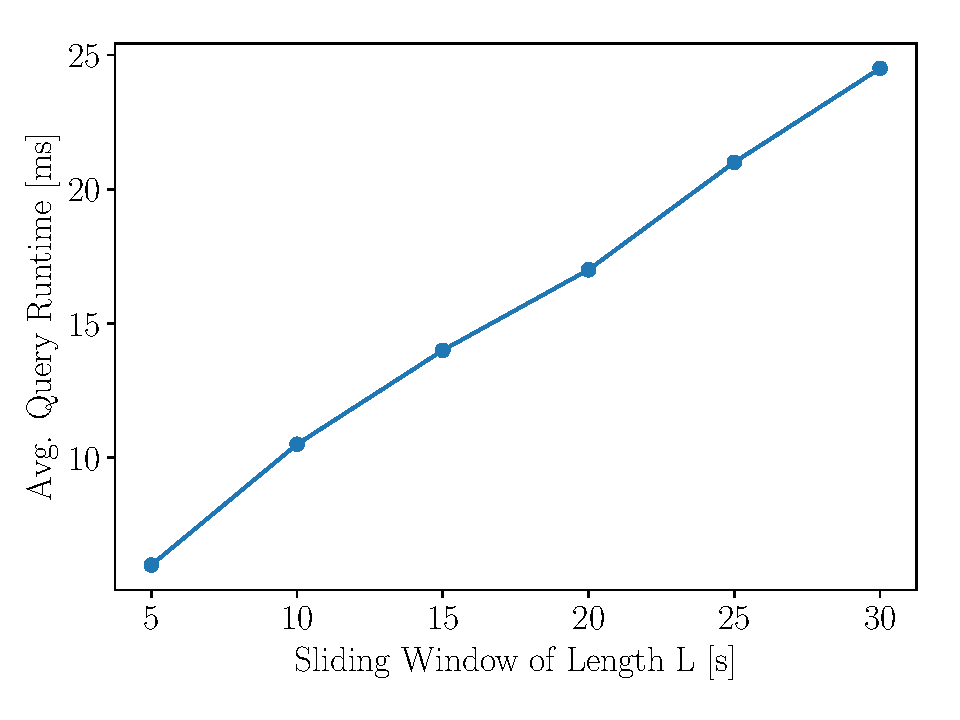
\includegraphics[width=8cm]{L_query_runtime_real}
    \caption{}
    \label{fig:L_query_runtime_real}
  \end{subfigure}
  \caption{Impact of Sliding Window of length $L$ on Query Runtime}
\end{figure}


\Cref{fig:trav_unprod_nodes_Ls_synthetic,fig:trav_unprod_nodes_Ls_real} show the
number of unproductive nodes the WAPI has traversed during query execution. As
expected, we observe greater sliding window lengths to cause an increase to the
rate of growth of unproductive nodes traversed by WAPI during query execution.
More volatile nodes imply an increase in unproductive nodes in the index.

\begin{figure}
  \centering
  \begin{subfigure}{0.49\linewidth}
    \centering
    Synthetic
  \end{subfigure}
  \begin{subfigure}{0.49\linewidth}
    \centering
    Real World
  \end{subfigure}
  \begin{subfigure}{0.49\linewidth}
    \centering
    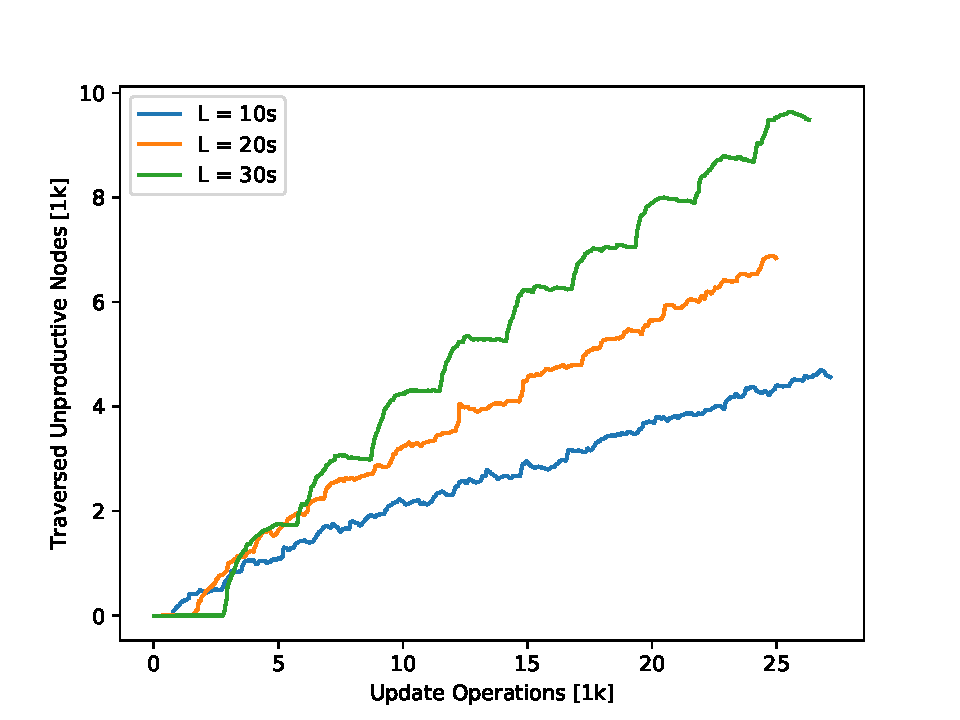
\includegraphics[width=8cm]{trav_unprod_nodes_Ls_synthetic}
    \caption{}
    \label{fig:trav_unprod_nodes_Ls_synthetic}
  \end{subfigure}
  \begin{subfigure}{0.49\linewidth}
    \centering
    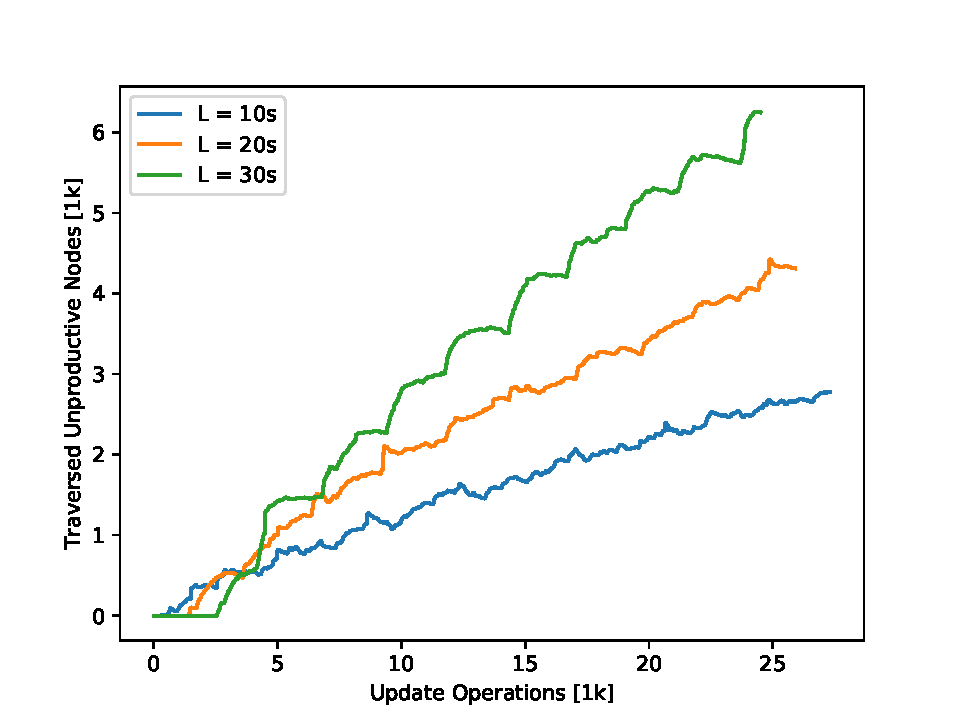
\includegraphics[width=8cm]{trav_unprod_nodes_Ls_real}
    \caption{}
    \label{fig:trav_unprod_nodes_Ls_real}
  \end{subfigure}
  \begin{subfigure}{0.49\linewidth}
    \centering
    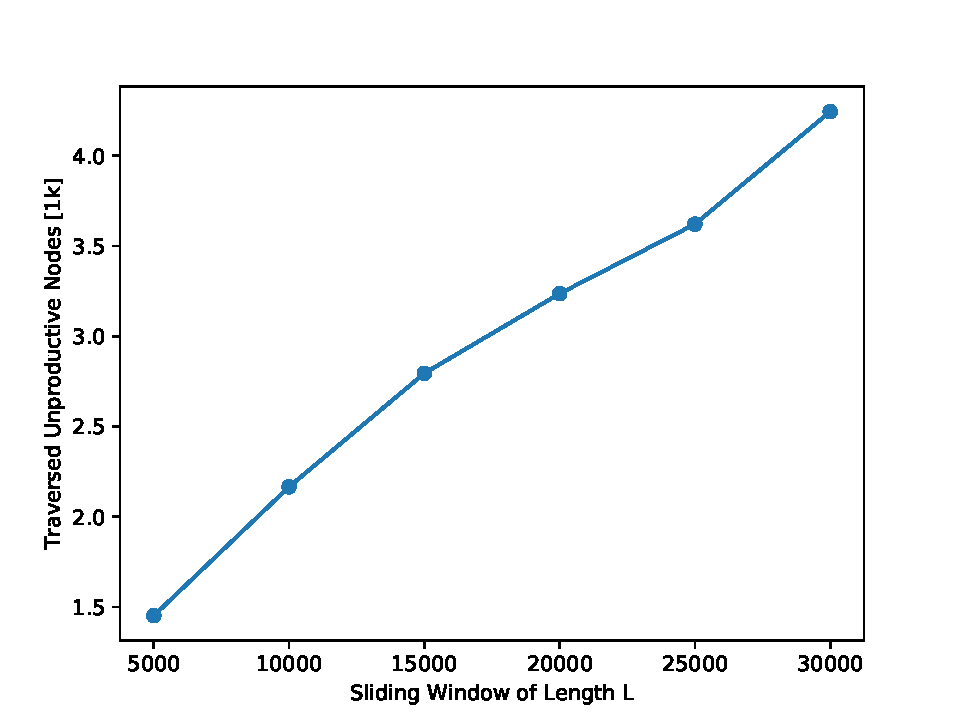
\includegraphics[width=8cm]{L_unprod_nodes_synthetic}
    \caption{}
    \label{fig:L_trav_unprod_nodes_synthetic}
  \end{subfigure}
  \begin{subfigure}{0.49\linewidth}
    \centering
    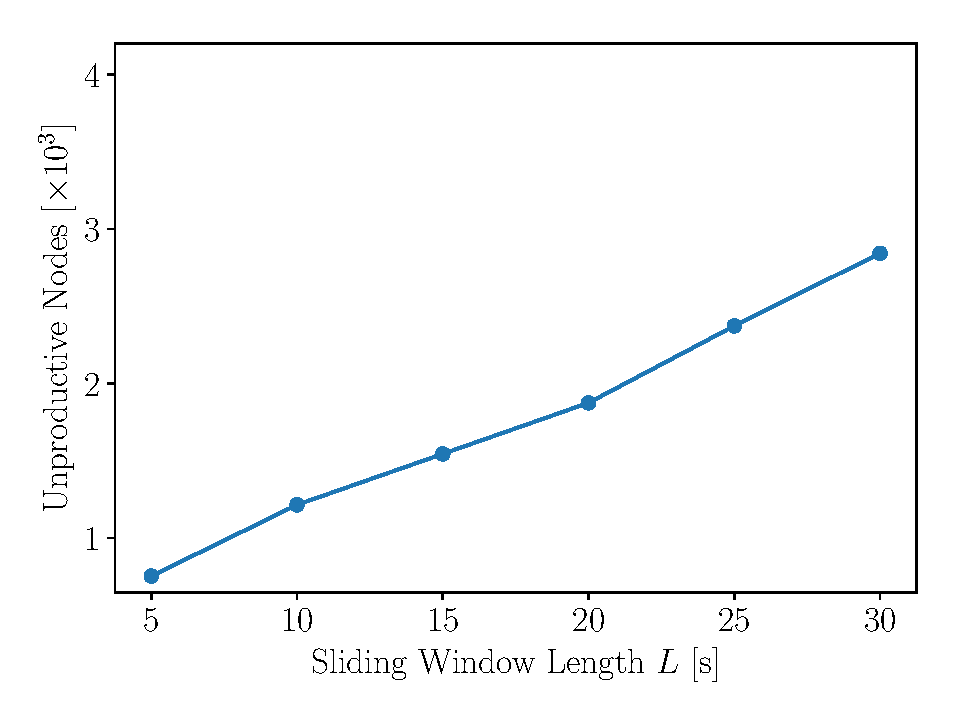
\includegraphics[width=8cm]{L_unprod_nodes_real}
    \caption{}
    \label{fig:L_trav_unprod_nodes_real}
  \end{subfigure}
  \caption{Impact of Sliding Window Length $L$ on Unproductive Nodes}
\end{figure}

Concluding, we see sliding window of length $L$ to be affecting query runtime.
Increasing $L$ does increase the likelihood of an index node become volatile.
More volatile nodes cause an increase in unproductive index nodes. Since the
WAPI has to traverse more index nodes during query execution, its query runtime
increases.

\section{Periodic Garbage Collection (GC)}

In the previous section, we saw how unproductive nodes slow down query
execution. To prevent unproductive nodes from accumulating in the index, we
clean the index periodically. Oak has a number of background processes that
maintain the database. We add a background job that periodically executes
garbage collection on Oak.

\Cref{algo:periodic_gc_wapi} takes an index node $n$ as parameter and prunes all
its unproductive descendants depth-first. The algorithm recursively traverses
the subtree rooted in $n$. If $n$ is a leaf node, is not matching and is not
volatile, it is pruned from the index. The depth-first tree traversal ensures
that the algorithm prunes a child before its parent node. This guarantees that
all unproductive nodes are pruned.

\begin{algorithm}
  \caption{CleanIndexWAPI}
  \DontPrintSemicolon
  \KwData{Index node $n$}
  % \vspace{2.6mm}
  \For{$c \in chd(n)$}{
    CleanIndexWAPI($c$)\;
  }
  \If{$leaf(n) \land \neg matching(n) \land \neg volatile(n)$}{
    delete node $n$\;
  }
  \label{algo:periodic_gc_wapi}
\end{algorithm}

\begin{figure}[h]
  \centering

  \begin{large}
    $$ G^0 \xrightarrow{\quad T_1 \quad} G^1$$
  \end{large}

\begin{subfigure}{0.30\textwidth}
  \centering \footnotesize{}{
    \begin{framed}
      \begin{forest}
        [
        [$\lambda$:$i$
        [$\lambda$:pub
        [$\lambda$:now
        [$\lambda$:$a$
        [$\lambda$:$b$
        [$\lambda$:$d$ \\ pub:now, align=center, base=bottom]
        ]
        [$\lambda$:$c$
        [$\lambda$:$e$]
        ]
        ]
        ]
        ]
        ]
        [$\lambda$:$a$
        [$\lambda$:$b$
        [$\lambda$:$d$ \\ pub:now, align=center, base=bottom]
        ]
        [$\lambda$:$c$
        [$\lambda$:$e$]
        ]
        ]
        ]
      \end{forest}
    \end{framed}
  } \footnotesize{ Snapshot $G^0$ }
\end{subfigure}
\begin{subfigure}{0.30\textwidth}
  \centering \footnotesize{
    \begin{framed}
      \begin{forest}
        [
        [$\lambda$:$i$
        [$\lambda$:pub
        [$\lambda$:now
        [$\lambda$:$a$
        [$\lambda$:$b$
        [$\lambda$:$d$ \\ pub:now, align=center, base=bottom]
        ]
        [,phantom]
        [,phantom]
        ]
        ]
        ]
        ]
        [$\lambda$:$a$
        [$\lambda$:$b$
        [$\lambda$:$d$ \\ pub:now, align=center, base=bottom]
        ]
        [$\lambda$:$c$
        [$\lambda$:$e$]
        ]
        ]
        ]
      \end{forest}
    \end{framed}
  } \footnotesize{ Snapshot $G^1$ }
\end{subfigure}

\vspace{3mm}
\caption*{
  Assume nodes \texttt{/i/pub/now/a/c/e} and \texttt{i/pub/now/a/c} are
  unproductive in snapshot $G^0$. Transaction $T_1$ is executed by the periodic
  garbage collector.
}
\caption{Garbage collection applied on Oak}
\label{fig:periodic_gc}
\end{figure}


\section{Query Time Pruning (QTP)}

\begin{algorithm}
  \caption{QueryQTP}
  \DontPrintSemicolon
  \KwData{Query $Q(k, v, m)$, where $k$ is a property, $v$ a value and $m$ a node.}
  \KwResult{A set of nodes satisfying $Q(k,v,m)$}
  $r \longleftarrow \emptyset$\;
  \For{$c \in chd(m)$}{
    $r \longleftarrow r \cup \text{QueryQTP}(k,v,c)$
    % \If{$n[k] = v$}{
      % $r \longleftarrow r \cup \{ *n \}$\;
    % }
  }
  $n \longleftarrow \texttt{/i/k/v/m}$\;
  \If{index node $n$ exists}{
    \uIf{$matching(n)$}{
      $r \longleftarrow r \cup \{m\}$\;
    }
    \ElseIf{$leaf(n) \land \neg volatile(n)$}{
      delete node $n$\;
    }
  }
  \Return{r}\;
  \label{algo:query_qtp_wapi}
\end{algorithm}

\section{Experimental Evaluation}

% In order to empirically evaluate and compare GC and QTP under a changing
% workload, a experiment harness has to be setup.

% datasets

% zipf distribution

% changing Workload

% parameters

\newpage

\bibliographystyle{abbrv}
\bibliography{thesis}

\end{document}
